%% Copyright 1998 Pepe Kubon
%%
%% `thes-short.tex' --- the example thesis, SHORT version, used
%%                     with  the `csthesis' package 
%% Use: latex thes-short to generate the DVI output, then 
%%      bibtex thes-short to generate the bibliography
%%      latex thes-short 
%%
%% You are allowed to distribute this file together with all files
%% mentioned in READ.ME.
%%
%% You are not allowed to modify its contents.
%%

\documentclass[11pt]{report}
%\documentclass[11pt,twoside]{report}%% for two-sided printing
\usepackage{pdfpages} 
\usepackage{anysize,fancyhdr,graphics}
\usepackage{csthesis}
\usepackage[titletoc]{appendix}%%Ensure word appendix appears in toc

\begin{document}
\setlength{\pdfpagewidth}{8.5in}
\setlength{\pdfpageheight}{11in}
%%% set switches
%\contentspagefalse  
%\figurespagetrue
%\tablespagetrue
%\dedicationpagetrue
%\quotationpagetrue
%\otherlistpagetrue

%%% front matter 
%% Copyright 1998 Pepe Kubon
%%
%% `titapp.tex' --- title and approval for thes-full.tex, thes-short-tex from
%%                  the `csthesis' bundle
%%
%% You are allowed to distribute this file together with all files
%% mentioned in READ.ME.
%%
%% You are not allowed to modify its contents.
%%

%%%%%%%%%%%%%%%%%%%%%%%%%%%%%%%%%%%%%%%%%%%%%
%
%   Title and approval pages
%
%%%%%%%%%%%%%%%%%%%%%%%%%%%%%%%%%%%%%%%%%%%%%

%%% title page

\title{Systematic Support of Parallel Bit Streams in LLVM}
\author{Meng Lin}
\qualification{B.Eng., University of Science and Technology of China, 2012}
\submitdate{Fall 2014}
\copyrightyear{2014}

%%% approval page


\chair{Dr.~Nick Sumner}

\signatory{Dr.~Robert D. Cameron,\\
       Professor,
       Computing Science,\\
       Simon Fraser University\\
       Senior Supervisor}

\signatory{Dr.~Thomas C. Shermer,\\
        Professor,
        Computing Science,\\
       %Simon Fraser University\\
       Supervisor}

\signatory{Dr.~Fred Popowich,\\
        Professor,
        Computing Science,\\
       %Simon Fraser University\\
       Supervisor}

\signatory{Dr.~Arthur (Ted) Kirkpatrick,\\
       Associate Director \& Professor,
       Computing Science, \\
       %Simon Fraser University\\
       External Examiner}

%%% generating title and approval pages
\beforepreface

 %% title, approval

%% Partial Copyright License (PCL)
\newpage 			
\addcontentsline{toc}{chapter}{Partial Copyright License}
\mbox{}
\makeatletter
\AddToShipoutPictureBG*{
            \setlength{\@tempdimc}{.06\paperheight}
            \setlength{\unitlength}{1pt}
           \put(\strip@pt\@tempdimb,\strip@pt\@tempdimc){
	\includegraphics{PCL_Declaration_2011.pdf}
	} 
} 
\makeatother
\newpage

%% Copyright 1998 Pepe Kubon
%%
%% `abstract.tex' --- abstract for thes-full.tex, thes-short-tex from
%%                    the `csthesis' bundle
%%
%% You are allowed to distribute this file together with all files
%% mentioned in READ.ME.
%%
%% You are not allowed to modify its contents.
%%

%%%%%%%%%%%%%%%%%%%%%%%%%%%%%%%%%%%%%%%%%%%%%%%%%
%
%       Abstract 
%
%%%%%%%%%%%%%%%%%%%%%%%%%%%%%%%%%%%%%%%%%%%%%%%%

\prefacesection{Abstract}
Here you put the abstract of the thesis.














 %% abstract
%% Copyright 1998 Pepe Kubon
%%
%% `dedquot.tex' --- dedication and quotation for thes-full.tex from
%%                   the `csthesis' bundle
%%
%% You are allowed to distribute this file together with all files
%% mentioned in READ.ME.
%%
%% You are not allowed to modify its contents.
%%

%%%%%%%%%%%%%%%%%%%%%%%%%%%%%%%%%%%%%%%%%%%%%
%
%   Dedication/Quotation pages
%
%%%%%%%%%%%%%%%%%%%%%%%%%%%%%%%%%%%%%%%%%%%%%

\dedication{To whomever whoever reads this!}
\thesquot{%
``Don't worry, Gromit. Everything's under control!''\\[5pt]%
--- The Wrong Trousers, \textsc{Aardman Animations}, 1993%
}

%%% generate pages
\dedicquotation
 %% dedication and quotation, if any 
%% Copyright 1998 Pepe Kubon
%%
%% `ack.tex' --- aknowledgments for thes-full.tex, thes-short-tex from
%%               the `csthesis' bundle
%%
%% You are allowed to distribute this file together with all files
%% mentioned in READ.ME.
%%
%% You are not allowed to modify its contents.
%%

%%%%%%%%%%%%%%%%%%%%%%%%%%%%%%%%%%%%%%%%%%%
%
%       Acknowledgment
%
%%%%%%%%%%%%%%%%%%%%%%%%%%%%%%%%%%%%%%%%%%

\prefacesection{Acknowledgments}

It is a great honor and pleasure for me to have my Master study in Simon Fraser University. I would like to give a big thank to Dr. Robert Cameron for all of his earnest instructions. I learnt a lot from him during these two years.

I would also like to thank Dr. Nick Sumner for his deep knowledge on LLVM and his great patience in assisting my thesis work. I would like to thank Dr. Thomas Shermer and Dr. Fred Popowich for early feedback on my thesis draft. I would like to give another big thank to Ken Herdy, who gave me a lot of support in those late nights in the lab. Nigel Medforth helped me with the experiments on icgrep as well as many instructions on the Parabix tool chain. Linda Lin helped me on Parabix tools too.

I would like to thank all the committee members for their precious time spent on my thesis. I would like to thank Simon Fraser University and Dr. Cameron again for providing me this awesome chance of studying computing science in Canada as well as providing financial support. I would like to thank my parents and all my friends in Canada that encouraged me and supported me during this journey.












 %%  acknowledgments

%%%  generate contents, lists of figures, etc.
\lists

%%% prepare main section
\beforetext

%%% main matter
%%%%%%%%%%%%%%%%%%%%%%%%%%%%%%%%%%%%%%%%%%%%%%%%%
%
%       Chapter 1
%
%%%%%%%%%%%%%%%%%%%%%%%%%%%%%%%%%%%%%%%%%%%%%%%%

\chapter{Introduction}
\label{one}

Nowadays Single Instruction Multiple Data (SIMD) instructions are broadly built in for most commodity processors. Compared with the traditional Single Instruction Single Data (SISD) instructions, SIMD provides an intra-register form of parallel computing by performing the same operation on many elements at the same time \cite{Fisher_phd}. SIMD instructions are widely used for multimedia processing, digital signal processing or other compute-intensive applications \cite{multimedia_simd, dsp_simd}.

The recent method of parallel bit streams (Parabix) accelerates text processing using SIMD instructions, in applications such as UTF-8 to UTF-16 transcoding \cite{rob_u8u16, rob_u8u16_techreport}, XML parsing \cite{medforth_icxml, rob_xml} and regular expression matching \cite{rob_regex}. For these applications, byte streams of the input text characters are first transposed into 8 bit streams, one for each bit value of the character byte, and then loaded into SIMD registers so that 128 or 256 consecutive code units can be processed at once \cite{inductive_doubling_principle}. SIMD bitwise logic, shift operations, bit scans and other bit-based operations form the foundation of this programming model.

Although Parabix applications achieve substantial acceleration compared to sequential (SISD) equivalents, the Parabix tool chain needs to handle SIMD programming carefully. It is challenging for the following two major reasons:

\begin{enumerate}
  \item SIMD instruction varies greatly among different instruction-set architectures (ISAs) which makes it hard to write portable SIMD programs. Some operations in Intel SSE may not exist in PowerPC AltiVec and vice versa. For example, integer comparison intrinsic $pcmpgtq$ in SSE4 does not have correspondence in PowerPC AltiVec.
  \item Even within one specific SIMD instruction set, most operations are only available for some pre-chosen data sizes. This is referred as "sparse instruction set" in \cite{hybrid_simd_type_legalize} and they gave a good example: in Intel SSE4, to shift-left a vector was implemented, but to shift-right was not. The 32-bit and 16-bit shift operations were available, but 64-bit shift was not \cite{hybrid_simd_type_legalize}.
\end{enumerate}

The current Parabix tool chain uses the Inductive Doubling Instruction Set Architecture (IDISA) as an idealized computing model to overcome these two difficulties. Based on this model a library with the same name has been developed. It works well, but still has two shortcomings:

\begin{enumerate}
  \item IDISA requires different header files for different architectures. Although it has a uniform API for portability, each header depends heavily on target-specific implementation details to provide the best implementation of each operation.
  \item The IDISA generator \cite{hua_idisa} chooses the best implementation within the scope of a single function. This may be not the best when considering the context of this function. For example, when performing addition, we may know all the high bits of each field in a SIMD register is zero, making simplification possible.
\end{enumerate}

This motivates us to find a better back end and currently, the most promising back end framework is LLVM\@. LLVM promises to enable out-sourcing of low-level and target-specific aspects of code generation \cite{llvm_ghc, chris_msthesis}. Switching to LLVM back end benefits Parabix tool chain for the following:

\begin{enumerate}
  \item LLVM provides a target-independent intermediate representation (IR) with a vector-of-integer type system that matches IDISA requirement closely. Parabix operations can be expressed with IR and hence can be ported, in principle, to any platform that LLVM supports, including X86, ARM, PowerPC, MIPS, SPARC and many more.
  \item LLVM provides inter-procedural, whole program analysis and optimization \cite{llvm_cgo04}. By built-in type system in the low level representation, LLVM keeps more static information to the back end and help optimize Parabix operation with meaningful context.
  \item LLVM provides just-in-time compilation which allows runtime source generation. This is critical to some applications such as regular expression matching, which generates sequence of Parabix operations on the fly according to the input regular expression.
\end{enumerate}

However, the native back end of LLVM has a number of gaps in its support for parallel bit streams. SIMD support for 2-bit and 4-bit field width are not available; 1-bit field width is supported slowly. Packing high bits on 16-bit field width which is one of the four key elements in the IDISA model and critical for transposition does not lower to proper machine code on X86. In this thesis, we extend LLVM to systematically support parallel bit streams and achieve high-performance code generation on the X86 target. We make the following contributions:

\begin{itemize}
  \item We port the critical Parabix operations to the LLVM back end thus bringing all the benefit of LLVM discussed above into the Parabix technology.
  \item We redefine type legality in LLVM and extend LLVM type system with the inductive doubling principle so that vectors of small element type are properly supported.
  \item We insert logic in the LLVM back end to recognize and handle key Parabix operations. This allows efficient code generation while keeping the whole source code in target-independent IR\@.
  \item We add a dedicated LLVM intrinsic for the long stream addition and enable high-performance chained addition on the unbounded integer model which can be applied in broader applications.
  \item We evaluate the new LLVM back end with both micro benchmarks on single Parabix operation and application level profiles. We get the performance on X86 platform as good as the well-tuned IDISA library.
\end{itemize}

The remainder of this thesis is organized as follows. Chapter~\ref{two} provides a quick review of Parabix and LLVM\@. Chapter~\ref{three} shows the overall design goal; examples of the IR implementation are presented and compared with the IDISA library. Algorithms for machine code generation is discussed in Chapter~\ref{four} and the implementation details is in Chapter~\ref{five}. Chapter~\ref{six} evaluates our work with both per-instruction benchmarks and application level profiles. Chapter~\ref{seven} gives the conclusion.

 
%%%%%%%%%%%%%%%%%%%%%%%%%%%%%%%%%%%%%%%%%%%%%%%%%
%
%     Chapter 2
%
%%%%%%%%%%%%%%%%%%%%%%%%%%%%%%%%%%%%%%%%%%%%%%%%

\chapter{Background}
\label{two}

\section{SIMD and SWAR}
SIMD is a parallel computing concept that performs the same instruction on different data to exploit data parallelism. Most of today's commodity processors supports SIMD within a register (SWAR) and in the SWAR model, SIMD operations are applied within general-purpose or special registers and these registers are often partitioned into fields. Operations on each field are independent from any other fields, which means for example, carry bits generated by addition would not pass to the next field.

The other important feature of the SWAR model is that the partition is not physical but rather a logical view of the register, so that different views are available on the same register. For a 128-bit SIMD register, a valid partition can be sixteen 8-bit fields as well as four 32-bit fields. There is no penalty from switching the logical view and it is important since it enables the inductive doubling principle we would discuss later.

However, since the SWAR instruction sets for different platforms are developed independently and operations available are determined mostly by the application requirements, different platform has different SWAR implementation, and the available instructions set are often sparse in the sense that not every power-of-two field width are supported \cite{hybrid_simd_type_legalize}.

\subsection{Commercial SIMD Instructions Sets}
Some popular SIMD instructions sets are listed here:
\begin{itemize}
  \item Intel MultiMedia eXtension (MMX). It defines eight 64-bit registers known as MM0 to MM7 which are aliases of the existing IA-32 Floating-Point Unit (FPU) stack registers. MMX only provides integer operations for early graphical applications thus is not a general purpose instruction set for SIMD programming \cite{hua_idisa}.
  \item Intel Streaming SIMD Extensions (SSE) series. SSE extends the MMX instructions set and introduces eight new independent 128-bit SIMD registers known as XMM0 to XMM7. Its successor SSE2 adds a rich set of integer instructions to the 128-bit XMM registers which makes it a useful SIMD programming model. AMD added support for SSE2 in its AMD64 architecture soon after the Intel released SSE2 thus in effect making SSE2 broadly available across the desktop computers. We would use SSE2 as our main instructions set target for 128-bit registers. Intel then released SSE3, SSSE3, SSE4 and AMD released SSE4a as the following SSE generations.
  \item Intel Advanced Vector Extensions (AVX). AVX extends the size of SIMD registers from 128 bits to 256 bits and introduces 16 new registers YMM0 to YMM15. It fully supports SSE instructions and more importantly, shifts the two-operand operations towards the non-destructive three-operand form, which would preserve the content in operand registers and reduce the potential movement of data between registers. AVX supports a number of floating point operations on 256-bit registers and its successor AVX2 fills the gap of integer operations and ensures the transition from SSE to AVX instructions with the same programming model. AVX2 is available on the Intel Haswell architecture, and we use it as our main 256-bit target. AVX512 as the next generation AVX has been announced to support 512-bit SIMD registers.
  \item ARM NEON\@. ARM as a popular mobile platform introduces its own SIMD extension named NEON in their Cortex-A series processors. It has thirty-two 64-bit registers (D0 to D31) as well as sixteen 128-bit registers (Q0 to Q15). In fact, $D_{2 \times i}$ and $D_{2 \times i + 1}$ are mapped to the same physical location of the register $Q_i$ and some operations like multiplication on the 64-bit D registers can return result in the 128-bit Q register \cite{hua_idisa}. NEON supports the field width of 8 bits, 16 bits, 32 bits and 64 bits integer operations as well as 32-bit floating point operations.
\end{itemize}

\section{Parabix Technology}
Parabix technology is a programming framework for high-performance text processing that can utilize both SIMD and multi-core parallel processing facility. It is built on top of the parallel bit streams concept. Byte-oriented input stream is first transposed into 8 bit streams with each stream corresponds to one bit location in the byte stream. For encodings that requires more than one byte, more bit streams can be introduced and in each bit stream, we would have 1 bit of the code unit from the input. Figure~\ref{figure:streams} gives an example of the transposition, $B_0$ to $B_7$ are the bit streams of the ASCII encoded input data and zero bits are marked as periods (.) for clarity.

\begin{figure}[tbh]
\begin{center}
\begin{tabular}{cr}\\
input data  & \verb`a453z--b3z--az--a12949z--ca22z7--`\\
$B_7$ & \verb`.................................`\\
$B_6$ & \verb`1...1..1.1..11..1.....1..11..1...`\\
$B_5$ & \verb`111111111111111111111111111111111`\\
$B_4$ & \verb`.1111...11...1...111111....1111..`\\
$B_3$ & \verb`....111..111.111...1.1111....1.11`\\
$B_2$ & \verb`.11..11...11..11....1..11.....111`\\
$B_1$ & \verb`...11..111...1....1...1..1.1111..`\\
$B_0$ & \verb`1.11.11.1.111.1111.1.1.1111...111`\\
\verb:[a]: & \verb`1...........1...1.........1......`\\
\verb:[z9]: & \verb`....1....1...1.....1.11......1...`\\
\verb:[0-9]: & \verb`.111....1........11111.....11.1..`
\end{tabular}
\end{center}
\caption[Basis and Character Class Streams]{Basis and Character Class Streams. Cited from \cite{rob_regex}.}
\label{figure:streams}
\end{figure}

After the transposition, the character class bit streams would be generated using bitwise logic, e.g.\ \verb:[a]:, \verb:[z9]: and \verb:[0-9]: in the figure. With SIMD operations on the 128-bit register, 128 input code unit can be classified at the same time. Parabix defines a set of primitives on the arbitrary length bit stream, called the \textit{Pablo Language} which is usually applied on the character class bit streams to generate a number of \textit{Marker Streams}. Marker Streams mark meaningful locations such as where a tag starts and ends in the XML document and matching positions of a partial regular expression. A simple counting or scanning through the marker streams are usually the final step in the Parabix technology.

Some useful Pablo primitives are listed as the following \cite{rob_xml_2011}:
\begin{enumerate}
    \item Bitwise logic: AND, OR, XOR and NOT on arbitrary length bit stream.
    \item Advance: shift forward the whole bit stream for 1 bit. In a little ending system, shift forward is to shift left because the bytes that comes first in the input stream resides in the lower memory address.
    \item ScanThru: $s(M, C)$ denotes the operation of scanning from the marker stream $M$ as the initial positions through the spans of ones in the stream $C$. Figure~\ref{figure:scanthru} shows an example of it.
      \[ s(M, C) = (M + C) \land \lnot C \]
      One example of ScanThru is in XML well-formedness checking, to check if a {\tt <tag>} is written in correct syntax, $M$ would mark all the start positions of tags e.g.\ the next position after the opening angle bracket ({\tt <}) and $C$ is the marker stream for all legal tag content. $s(M, C)$ should mark all the positions of the closing angle bracket ({\tt >}) which close tags. Say $M_0$ denotes the character class of {\tt >}, then if $s(M, C) \land \lnot M_0$ is not all zero, some tag is not closed properly with the {\tt >} symbol. Note that all the tags in the stream are checked at once in parallel in the unbounded bit streams model.
    \item MatchStar: $m(M, C)$ returns all positions that can be reached by scanning from the initial positions marked in $M$ along the spans of ones in the stream $C$ for zero or more steps. MatchStar gets its name from the star operator (*) in the regular expression and it also has important application in the long stream addition. Figure~\ref{figure:matchstar} shows an example of it.
\end{enumerate}

\begin{figure}[tbh]
\begin{center}
\begin{tabular}{cr}\\
input data  & \verb`----173942---654----1----49731----321--`\\
$M_0$ &                          \verb`....1........1......1......1...........`\\
$D = $\verb:[0-9]: &             \verb`....111111...111....1....11111....111..`\\
$M_0 + D$ &                      \verb`..........1.....1....1...11...1...111..`\\
$M_1 = (M_0 + D) \wedge \neg D$ &\verb`..........1.....1....1........1........`
\end{tabular}
\end{center}
\caption[ScanThru Using Bitstream Addition and Mask]{ScanThru Using Bitstream Addition and Mask. Cited from \cite{rob_xml_2011} and slightly modified.}
\label{figure:scanthru}
\end{figure}

\begin{figure}[tbh]
\begin{center}
\begin{tabular}{cr}\\
input data  & \verb`a453z--b3z--az--a12949z--ca22z7--`\\
$M_1$ & \verb`.1...........1...1.........1.....`\\
$C = \text{\tt [0-9]}$ & \verb`.111....1........11111.....11.1..`\\
$T_0 = M_1 \wedge C$ & \verb`.1...............1.........1.....`\\
$T_1 = T_0 + C$ & \verb`....1...1.............1......11..`\\
$T_2 = T_1 \oplus C$ & \verb`.1111............111111....111...`\\
$M_2 = T_2 \vee M_1$ & \verb`.1111........1...111111....111...`
\end{tabular}
\end{center}
\caption[MatchStar Using Bitstream Addition and Mask]{MatchStar primitive, where $M_2 = \text{MatchStar}(M_1, C)$. Cited from \cite{rob_regex}.}
\label{figure:matchstar}
\end{figure}

Pablo Language are defined over unbounded bit streams which of course need to be translated into a block-at-a-time processing for real applications \cite{rob_regex}. The Pablo compiler is used here for the translation and it will take care of the carry bits across block boundaries with a carry queue. A block-at-a-time C++ code would be generated as a result.

\subsection{IDISA Library}
To actually execute the C++ code, a set of runtime library is necessary. Dr. Cameron proposed the Inductive Doubling Instructions Set Architecture in \cite{inductive_doubling_principle} and claimed significant instruction count reduction in core parallel bit stream algorithm. As he wrote, "inductive doubling refers to a general property of certain kinds of algorithm that systematically double the values of field widths or other data attributes with each iteration."\cite{inductive_doubling_principle}. There are four key elements of this architecture:
\begin{itemize}
    \item A core set of binary functions on SIMD registers, for all field width equals to $2^k$. To work with parallel bit streams, the operation ADD, SUB, SHL, SRL and ROTL (rotate left) comprise the set.
    \item A set of \textit{half-operand modifiers} that make possible the inductive processing of field width $2W$ in terms of combinations of field width $W$. These modifiers select either the lower half of the field or the higher half.
    \item Packing operations that compress two vectors of field width $W$ into one vector of field width $W/2$. E.g.\ collecting all the higher half bits of fields from two vectors into one.
    \item Merging operations that produce one vector of field width $W$ with two vectors of field width $W/2$.
\end{itemize}

A C++ library is then developed after this model and it is called the IDISA library. To be clear, in the following sessions the abstract architecture will be called the IDISA model to distinguish from the IDISA library. An interesting fact about the IDISA library is that it is actually generated automatically from a pool of strategies to avoid duplicated human work among different targets. When targeting at a new platform, a set of machine intrinsic will be mapped to proper instructions in the IDISA model. This would be sparse that many other operations needed by the model are still not available. The IDISA library generator could fill the gaps with a pool of strategies which basically tells how to implement instruction C given instruction A and B are available. Multiple strategies for the same instruction may exist and the generator would choose based on least instruction count mechanism \cite{hua_idisa}.

\begin{figure}[ht!]
\centering
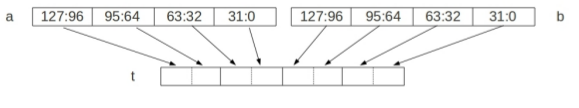
\includegraphics[width=130mm]{draw/horizontal.png}
\caption[Horizontal Operations in IDISA]{The logic of IDISA Horizontal Operations, cited from \cite{hua_idisa}.}
\label{figure:horizontal}
\end{figure}

\begin{figure}[ht!]
\centering
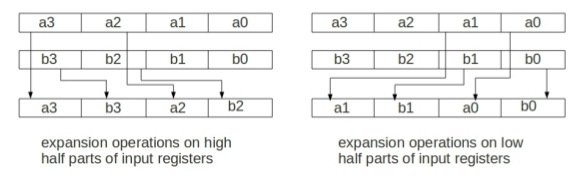
\includegraphics[width=130mm]{draw/expansion.png}
\caption[Expansion Operations in IDISA]{The logic of IDISA Expansion Operations, cited from \cite{hua_idisa}.}
\label{figure:expansion}
\end{figure}

The IDISA library divides SIMD operations in the following categories \cite{idisa_webpage}:
\begin{itemize}
    \item Vertical Operations (Template Class {\tt simd<w>}): Most common SIMD operations between two registers and {\tt w} is the field width. E.g.\ {\tt simd<8>::add(A, B)} aligns registers A and B vertically and adds up the aligned 8-bit fields. Different fields are independent of each other.
    \item Horizontal Operations (Template Class {\tt hsimd<w>}): Operations like packing align the two operands horizontally, extract a portion of the bits in operands and concatenate into one full SIMD register. (Figure~\ref{figure:horizontal})
    \item Expansion Operations (Template Class {\tt esimd<w>}): Operations that double the width of fields like merging which would take the higher 64 bits of the two operands (A and B), concatenate the first field from A and the first field from B and get a new field with the width doubled. Do the same to the following fields until a full SIMD register C is generated. (Figure~\ref{figure:expansion})
    \item Field Movement Operations (Template Class {\tt mvmd<w>}): Operations that copy and move the entire fields. The content of these fields would not change.
\end{itemize}

The IDISA library claims to have better performance compared to the hand-written libraries and it is the main competitor of our LLVM back end.

\subsection{Critical Parabix Operations}
There are at least three critical Parabix operations that can be the performance bottleneck and need special attention:
\begin{itemize}
    \item Transposition. The first step of every Parabix application and can be the primary overhead of some Parabix application. There are two major algorithms: the ideal three-stage implementation and the byte-pack implementation. The byte-pack implementation utilize packing on 16 bit field width which is widely available on commodity processors while the ideal three-stage implementation was proved optimal in instruction count in the IDISA model. Details of these two algorithms can be found in \cite{inductive_doubling_principle}.
    \item Inverse transposition. For some applications like the UTF-8 to UTF-16 transcoding, parallel bit streams needs to be modified and translated back into byte streams, thus an inverse transposition is needed. As the inverse operation to the transposition, there are also two algorithms available which mirror the transposition algorithms. A detailed discussion can be found in \cite{rob_u8u16}.
    \item Long stream addition. Pablo compiler deal with addition between unbounded bit streams using chained long stream additions, which adds two numbers as wide as the SIMD register with a carry-in bit and generates a carry-out bit. The naive approach would be chaining 64-bit additions together to emulate 128-bit, 256-bit or 512-bit additions. The time complexity of the naive approach grows linearly with the SIMD register size and a better algorithm is proposed in \cite{rob_regex} which could adds up to 4096 bits wide integers in constant time. We would discuss this algorithm further in Chapter~\ref{four}.
\end{itemize}

Since they are performance critical, these operations would be used as the application level benchmarks in the evaluation section.

\section{LLVM Basics}
The \textit{Low Level Virtual Machine (LLVM)} is an open-source, well developed compiler tool that is dedicated to the compiler writers. It is proposed in 2000 with Lattner's Master thesis \cite{chris_msthesis} and is gaining popularity ever after. Today it is developed into a high-performance static compiler back end with just-in-time compilers and life-long program analysis and optimization, which means program analysis and optimization in compile time, link time and run time \cite{llvm_ghc, llvm_cgo04}. It supports a variety of targets from Intel X86, PowerPC to the ARM mobile platform and hides the low-level target-specific issues for the compiler writers. LLVM is now sponsored by companies like Google and Apple and it is likely to become the default back end choice that last a long time in this field.

LLVM uses the intermediate representation (IR) as its virtual instruction set and IR is used as not only the input code to the LLVM tool chain but also the internal representation for analysis and optimization passes. This enables the programmer to use LLVM as a pipeline and inspect output from each step. Although IR is low-level, it preserves high-level static information through the strong type system and its static single assignment (SSA) form. According to \cite{cytron1991efficiently}, SSA form guarantees only one assignment to every variable and would help calculate the high-level data flow. The main design goal of IR is to be low-level enough so that most programming language can target to it while maintaining the most high-level information to make aggressive back end optimization possible \cite{llvm_ghc}.

LLVM IR is target-independent and it provides powerful operations like shufflevector that can express most of the complex Parabix operations. The IR code are processed through the target-independent code generator and the machine code (MC) layer to become the native machine code. We will describe the code generation process in detail in the next section as it is the major piece of logic we extend for parallel bit streams.

\section{LLVM Target-Independent Code Generator}
The first stage for code generation is Instruction Selection, which translates LLVM code into the target-specific machine instructions. After that, there are machine level optimization like live-interval analysis and register allocation. We focus on Instruction Selection and it is done by the following steps \cite{llvm_code_gen} (we would describe each step in the following text):

\begin{itemize}
  \item Initial SelectionDAG Construction: generate SelectionDAG from LLVM IR.
  \item DAG Combine 1
  \item Legalize Types Phase
  \item Post Legalize Type DAG Combine
  \item Legalize Phase
  \item DAG Combine 2
  \item Instruction Select Phase
  \item Scheduling and Formation Phase
\end{itemize}

LLVM internally constructs a graph view of the input code called SelectionDAG where DAG is short for directed acyclic graph. Each node in the DAG represents an operation with an opcode, a number of operands and a number of return values. If the DAG node A uses the return value of the other DAG node B, an edge will be there from B to A. The SelectionDAG enables a large variety of very-low-level optimization and also benefits the instruction scheduling process by recording the instruction dependency in the graph.

There are DAG combine passes after the initial construction and each legalize phase\cite{llvm_code_gen}. We will explain "legality" in the next section. DAG combine passes clean up SelectionDAG with both general and machine-dependent strategies, making the work easier for initial constructor and legalizers: they can focus on generating accurate SelectionDAG, good and legal operations with no worries of the messy output.

Instruction Select Phase is the bulk of target-specific logic that translates a legal SelectionDAG into a new DAG of target code with pattern matching facility. For example, a node of floating point addition followed by a floating point multiplication could be merged into one FMADDS node on the target that supports floating point multiply-and-add (FMA) operations \cite{llvm_code_gen}.

The Scheduling and Formation Phase would assign an order to each target instruction following the target's constraints. After that, a list of MachineInstrs will be generated and the SelectionDAG is no longer needed.

\subsection{Vector Type and Legality}
SIMD data are grouped into vectors and LLVM uses the notion \verb|<N x iX>| to represent a vector of N elements, where each of the element is an integer of X bits \cite{llvm_lang_ref, hybrid_simd_type_legalize}. \verb|<N x iX>| is also denoted as $vNiX$ as $vNiX$ is the internal type name used in the LLVM source code; e.g.\ \verb|<4 x i32>| is the same with $v4i32$.

In LLVM IR, programmer can write any kind of vectors, even $v1024i3$, and those vectors may not be supported by the target machine. LLVM has the notion of a "legal" vs. "illegal". A type is legal for a target only if it is supported by some operation. In SelectionDAG, a DAG node is legal only if the target supports the operation and operands type. For example, $v16i8$ is legal on X86 SSE2 architecture, since the architecture supports ADD on 2 $v16i8$ vectors; but it does not support multiplication on 2 $v16i8$ vectors, so that the DAG node MUL on $v16i8$ is illegal. LLVM has Legalize Types and Legalize Operations Phases to turn illegal type or DAG into legal\cite{llvm_code_gen}.

Legalize type phase has three ways to legalize vector types\cite{hybrid_simd_type_legalize}: \textit{Scalarization}, \textit{Vector Widening} and \textit{Vector Element Promotion}.

\begin{itemize}
    \item \textbf{Scalarization} splits the vector into multiple scalars. It is often used for $v1iX$ as the edge case when LLVM is trying to split the incoming vector into sub vectors.
    \item \textbf{Vector Widening} adds dummy elements to make the vector fit the right register size. It will not change the type of the elements, e.g.\ $v4i8$ to $v16i8$.
    \item \textbf{Vector Element Promotion} preserves the number of elements, but promote the element type to a wider size, e.g.\ $v4i8$ to $v4i32$.
\end{itemize}

After the type legalization, we may still have illegal DAG node, such as multiplication on $v16i8$ for X86 SSE2 architecture; thus we need legalize operations phase. There are three strategies in this phase:

\begin{itemize}
    \item \textbf{Expansion}: Use another sequence of operations to emulate the operation. Expansion strategy is often general in the sense that it may use slow operations such as memory load and store, but it would generate native code with correct outcome.
    \item \textbf{Promotion}: Promote the operand type to a larger type that the operation supports.
    \item \textbf{Custom}: Write a target-specific code to implement the legalization. Similar to Expansion, but with a specific target in mind.
\end{itemize}

No illegal type should be introduced in the operation legalization which puts a limitation on the machine-independent legalize strategies: $i8$ is the minimum integer type on X86 and programmer needs to extend every integer less than 8 bits to $i8$ before returning it to the DAG\@. On the other hand DAG combine is different, you can choose the combine timing on your own. If you choose to combine before Legalize Types Phase, you can freely introduce illegal types into your combined results.


%%%  appendices, if any
\begin{appendices}
%% Copyright 1998 Pepe Kubon
%%
%% `appone.tex' --- 1st appendix for thes-full.tex, thes-short-tex from
%%                  the `csthesis' bundle
%%
%% You are allowed to distribute this file together with all files
%% mentioned in READ.ME.
%%
%% You are not allowed to modify its contents.
%%

%%%%%%%%%%%%%%%%%%%%%%%%%%%%%%%%%%%%%%%%%%%%%%%%%
%
%        Appendix 1
%
%%%%%%%%%%%%%%%%%%%%%%%%%%%%%%%%%%%%%%%%%%%%%%%%

\chapter{Appendices: Example Code From The IR Library}\label{app:one}

\section{Transposition With Byte-Pack Algorithm}
\label{appone:transposition}

\begin{lstlisting}
define <4 x i32> @packh_16(<4 x i32> %a, <4 x i32> %b) alwaysinline {
entry:
  %aa = bitcast <4 x i32> %a to <16 x i8>
  %bb = bitcast <4 x i32> %b to <16 x i8>
  %rr = shufflevector <16 x i8> %bb, <16 x i8> %aa, <16 x i32> <i32 1,
        i32 3, i32 5, i32 7, i32 9, i32 11, i32 13, i32 15, i32 17,
        i32 19, i32 21, i32 23, i32 25, i32 27, i32 29, i32 31>

  %rr1 = bitcast <16 x i8> %rr to <4 x i32>
  ret <4 x i32> %rr1
}

define <4 x i32> @packl_16(<4 x i32> %a, <4 x i32> %b) alwaysinline {
entry:
  %aa = bitcast <4 x i32> %a to <16 x i8>
  %bb = bitcast <4 x i32> %b to <16 x i8>
  %rr = shufflevector <16 x i8> %bb, <16 x i8> %aa, <16 x i32> <i32 0,
        i32 2, i32 4, i32 6, i32 8, i32 10, i32 12, i32 14, i32 16,
        i32 18, i32 20, i32 22, i32 24, i32 26, i32 28, i32 30>

  %rr1 = bitcast <16 x i8> %rr to <4 x i32>
  ret <4 x i32> %rr1
}

define <4 x i32> @ifh_1(<4 x i32> %cond, <4 x i32> %b, <4 x i32> %c)
alwaysinline {
entry:
  %not_cond = xor <4 x i32> %cond, <i32 -1, i32 -1, i32 -1, i32 -1>

  %t0 = and <4 x i32> %cond, %b
  %t1 = and <4 x i32> %not_cond, %c
  %r = or <4 x i32> %t0, %t1

  ret <4 x i32> %r
}

define <4 x i32> @srli_16(<4 x i32> %a, <8 x i16> %shift_mask)
alwaysinline {
entry:
  %aa = bitcast <4 x i32> %a to <8 x i16>
  %r0 = lshr <8 x i16> %aa, %shift_mask
  %rr = bitcast <8 x i16> %r0 to <4 x i32>
  ret <4 x i32> %rr
}

define <4 x i32> @slli_16(<4 x i32> %a, <8 x i16> %shift_mask)
alwaysinline {
entry:
  %aa = bitcast <4 x i32> %a to <8 x i16>
  %r0 = shl <8 x i16> %aa, %shift_mask
  %rr = bitcast <8 x i16> %r0 to <4 x i32>
  ret <4 x i32> %rr
}

define void @s2p_step_ir(<4 x i32> %s0, <4 x i32> %s1,
  <4 x i32> %hi_mask, <8 x i16> %shift_mask, <4 x i32>* %p0,
  <4 x i32>* %p1) alwaysinline {
entry:
  %t0 = call <4 x i32> @packh_16(<4 x i32> %s0, <4 x i32> %s1)
  %t1 = call <4 x i32> @packl_16(<4 x i32> %s0, <4 x i32> %s1)

  %t2 = call <4 x i32> @srli_16(<4 x i32> %t1, <8 x i16> %shift_mask)
  %q0 = call <4 x i32> @ifh_1(<4 x i32> %hi_mask, <4 x i32> %t0,
                              <4 x i32> %t2)
  %t3 = call <4 x i32> @slli_16(<4 x i32> %t0, <8 x i16> %shift_mask)
  %q1 = call <4 x i32> @ifh_1(<4 x i32> %hi_mask, <4 x i32> %t3,
                              <4 x i32> %t1)

  store <4 x i32> %q0, <4 x i32>* %p0
  store <4 x i32> %q1, <4 x i32>* %p1

  ret void
}

define <8 x i16> @const16_1() alwaysinline {
entry:
  ret <8 x i16> <i16 1, i16 1, i16 1, i16 1, i16 1, i16 1, i16 1, i16 1>
}

define <8 x i16> @const16_2() alwaysinline {
entry:
  ret <8 x i16> <i16 2, i16 2, i16 2, i16 2, i16 2, i16 2, i16 2, i16 2>
}

define <8 x i16> @const16_4() alwaysinline {
entry:
  ret <8 x i16> <i16 4, i16 4, i16 4, i16 4, i16 4, i16 4, i16 4, i16 4>
}

define <4 x i32> @himask_2() alwaysinline {
entry:
  ret <4 x i32> <i32 -1431655766, i32 -1431655766,
                 i32 -1431655766, i32 -1431655766>
}

define <4 x i32> @himask_4() alwaysinline {
entry:
  ret <4 x i32> <i32 -858993460, i32 -858993460,
                 i32 -858993460, i32 -858993460>
}

define <4 x i32> @himask_8() alwaysinline {
entry:
  ret <4 x i32> <i32 -252645136, i32 -252645136,
                 i32 -252645136, i32 -252645136>
}

define void @s2p_bytepack_ir(<4 x i32> %s0, <4 x i32> %s1, <4 x i32> %s2,
  <4 x i32> %s3, <4 x i32> %s4, <4 x i32> %s5, <4 x i32> %s6,
  <4 x i32> %s7, <4 x i32>* %p0, <4 x i32>* %p1, <4 x i32>* %p2,
  <4 x i32>* %p3, <4 x i32>* %p4, <4 x i32>* %p5, <4 x i32>* %p6,
  <4 x i32>* %p7) {
entry:
  %bit00224466_0 = alloca <4 x i32>, align 16
  %bit00224466_1 = alloca <4 x i32>, align 16
  %bit00224466_2 = alloca <4 x i32>, align 16
  %bit00224466_3 = alloca <4 x i32>, align 16
  %bit11335577_0 = alloca <4 x i32>, align 16
  %bit11335577_1 = alloca <4 x i32>, align 16
  %bit11335577_2 = alloca <4 x i32>, align 16
  %bit11335577_3 = alloca <4 x i32>, align 16
  %bit00004444_0 = alloca <4 x i32>, align 16
  %bit22226666_0 = alloca <4 x i32>, align 16
  %bit00004444_1 = alloca <4 x i32>, align 16
  %bit22226666_1 = alloca <4 x i32>, align 16
  %bit11115555_0 = alloca <4 x i32>, align 16
  %bit33337777_0 = alloca <4 x i32>, align 16
  %bit11115555_1 = alloca <4 x i32>, align 16
  %bit33337777_1 = alloca <4 x i32>, align 16

  %call10 = call <4 x i32> @himask_2()
  %call11 = call <8 x i16> @const16_1()
  call void @s2p_step_ir(<4 x i32> %s0, <4 x i32> %s1,
  <4 x i32> %call10,
  <8 x i16> %call11, <4 x i32>* %bit00224466_0,
  <4 x i32>* %bit11335577_0)
  %call14 = call <4 x i32> @himask_2()
  %call15 = call <8 x i16> @const16_1()
  call void @s2p_step_ir(<4 x i32> %s2, <4 x i32> %s3,
  <4 x i32> %call14,
  <8 x i16> %call15, <4 x i32>* %bit00224466_1,
  <4 x i32>* %bit11335577_1)
  %call18 = call <4 x i32> @himask_2()
  %call19 = call <8 x i16> @const16_1()
  call void @s2p_step_ir(<4 x i32> %s4, <4 x i32> %s5,
  <4 x i32> %call18,
  <8 x i16> %call19, <4 x i32>* %bit00224466_2,
  <4 x i32>* %bit11335577_2)
  %call22 = call <4 x i32> @himask_2()
  %call23 = call <8 x i16> @const16_1()
  call void @s2p_step_ir(<4 x i32> %s6, <4 x i32> %s7,
  <4 x i32> %call22,
  <8 x i16> %call23, <4 x i32>* %bit00224466_3,
  <4 x i32>* %bit11335577_3)
  %p23 = load <4 x i32>* %bit00224466_0, align 16
  %p24 = load <4 x i32>* %bit00224466_1, align 16
  %call24 = call <4 x i32> @himask_4()
  %call25 = call <8 x i16> @const16_2()
  call void @s2p_step_ir(<4 x i32> %p23, <4 x i32> %p24,
  <4 x i32> %call24,
  <8 x i16> %call25, <4 x i32>* %bit00004444_0,
  <4 x i32>* %bit22226666_0)
  %p25 = load <4 x i32>* %bit00224466_2, align 16
  %p26 = load <4 x i32>* %bit00224466_3, align 16
  %call26 = call <4 x i32> @himask_4()
  %call27 = call <8 x i16> @const16_2()
  call void @s2p_step_ir(<4 x i32> %p25, <4 x i32> %p26,
  <4 x i32> %call26,
  <8 x i16> %call27, <4 x i32>* %bit00004444_1,
  <4 x i32>* %bit22226666_1)
  %p27 = load <4 x i32>* %bit11335577_0, align 16
  %p28 = load <4 x i32>* %bit11335577_1, align 16
  %call28 = call <4 x i32> @himask_4()
  %call29 = call <8 x i16> @const16_2()
  call void @s2p_step_ir(<4 x i32> %p27, <4 x i32> %p28,
  <4 x i32> %call28,
  <8 x i16> %call29, <4 x i32>* %bit11115555_0,
  <4 x i32>* %bit33337777_0)
  %p29 = load <4 x i32>* %bit11335577_2, align 16
  %p30 = load <4 x i32>* %bit11335577_3, align 16
  %call30 = call <4 x i32> @himask_4()
  %call31 = call <8 x i16> @const16_2()
  call void @s2p_step_ir(<4 x i32> %p29, <4 x i32> %p30,
  <4 x i32> %call30,
  <8 x i16> %call31, <4 x i32>* %bit11115555_1,
  <4 x i32>* %bit33337777_1)

  %p31 = load <4 x i32>* %bit00004444_0, align 16
  %p32 = load <4 x i32>* %bit00004444_1, align 16
  %call32 = call <4 x i32> @himask_8()
  %call33 = call <8 x i16> @const16_4()
  call void @s2p_step_ir(<4 x i32> %p31, <4 x i32> %p32,
  <4 x i32> %call32,
  <8 x i16> %call33, <4 x i32>* %p0, <4 x i32>* %p4)
  %p33 = load <4 x i32>* %bit11115555_0, align 16
  %p34 = load <4 x i32>* %bit11115555_1, align 16
  %call36 = call <4 x i32> @himask_8()
  %call37 = call <8 x i16> @const16_4()
  call void @s2p_step_ir(<4 x i32> %p33, <4 x i32> %p34,
  <4 x i32> %call36,
  <8 x i16> %call37, <4 x i32>* %p1, <4 x i32>* %p5)
  %p35 = load <4 x i32>* %bit22226666_0, align 16
  %p36 = load <4 x i32>* %bit22226666_1, align 16
  %call40 = call <4 x i32> @himask_8()
  %call41 = call <8 x i16> @const16_4()
  call void @s2p_step_ir(<4 x i32> %p35, <4 x i32> %p36,
  <4 x i32> %call40,
  <8 x i16> %call41, <4 x i32>* %p2, <4 x i32>* %p6)
  %p37 = load <4 x i32>* %bit33337777_0, align 16
  %p38 = load <4 x i32>* %bit33337777_1, align 16
  %call44 = call <4 x i32> @himask_8()
  %call45 = call <8 x i16> @const16_4()
  call void @s2p_step_ir(<4 x i32> %p37, <4 x i32> %p38,
  <4 x i32> %call44,
  <8 x i16> %call45, <4 x i32>* %p3, <4 x i32>* %p7)

  ret void
}

\end{lstlisting}

\section{Transposition With Ideal 3-Stage Algorithm}
\label{appone:transposition_ideal}
\begin{lstlisting}
define <4 x i32> @packh_8(<4 x i32> %a, <4 x i32> %b) alwaysinline {
entry:
  %aa = bitcast <4 x i32> %a to <32 x i4>
  %bb = bitcast <4 x i32> %b to <32 x i4>
  %rr = shufflevector <32 x i4> %bb, <32 x i4> %aa, <32 x i32>
   <i32 1, i32 3, i32 5, i32 7,  i32 9,  i32 11,  i32 13,  i32 15,
   i32 17,  i32 19,  i32 21,  i32 23,  i32 25,  i32 27,  i32 29,
   i32 31,  i32 33,  i32 35,  i32 37,  i32 39,  i32 41,  i32 43,
   i32 45,  i32 47,  i32 49,  i32 51,  i32 53,  i32 55,  i32 57,
   i32 59,  i32 61,  i32 63>

  %rr1 = bitcast <32 x i4> %rr to <4 x i32>
  ret <4 x i32> %rr1
}

define <4 x i32> @packl_8(<4 x i32> %a, <4 x i32> %b) alwaysinline {
entry:
  %aa = bitcast <4 x i32> %a to <32 x i4>
  %bb = bitcast <4 x i32> %b to <32 x i4>
  %rr = shufflevector <32 x i4> %bb, <32 x i4> %aa, <32 x i32>
   <i32 0,  i32 2,  i32 4,  i32 6,  i32 8,  i32 10,  i32 12,  i32 14,
   i32 16,  i32 18,  i32 20,  i32 22,  i32 24,  i32 26,  i32 28,
   i32 30,  i32 32,  i32 34,  i32 36,  i32 38,  i32 40,  i32 42,
   i32 44,  i32 46,  i32 48,  i32 50,  i32 52,  i32 54,  i32 56,
   i32 58,  i32 60,  i32 62>

  %rr1 = bitcast <32 x i4> %rr to <4 x i32>
  ret <4 x i32> %rr1
}

define <4 x i32> @packh_4(<4 x i32> %a, <4 x i32> %b) alwaysinline {
entry:
  %aa = bitcast <4 x i32> %a to <64 x i2>
  %bb = bitcast <4 x i32> %b to <64 x i2>
  %rr = shufflevector <64 x i2> %bb, <64 x i2> %aa, <64 x i32> <i32 1,
   i32 3,  i32 5,  i32 7,  i32 9,  i32 11,  i32 13,  i32 15,  i32 17,
   i32 19,  i32 21,  i32 23,  i32 25,  i32 27,  i32 29,  i32 31,
   i32 33,  i32 35,  i32 37,  i32 39,  i32 41,  i32 43,  i32 45,
   i32 47,  i32 49,  i32 51,  i32 53,  i32 55,  i32 57,  i32 59,
   i32 61,  i32 63,  i32 65,  i32 67,  i32 69,  i32 71,  i32 73,
   i32 75,  i32 77,  i32 79,  i32 81,  i32 83,  i32 85,  i32 87,
   i32 89,  i32 91,  i32 93,  i32 95,  i32 97,  i32 99,  i32 101,
   i32 103,  i32 105,  i32 107,  i32 109,  i32 111,  i32 113,
   i32 115,  i32 117,  i32 119,  i32 121,  i32 123,  i32 125,  i32 127>

  %rr1 = bitcast <64 x i2> %rr to <4 x i32>
  ret <4 x i32> %rr1
}

define <4 x i32> @packl_4(<4 x i32> %a, <4 x i32> %b) alwaysinline {
entry:
  %aa = bitcast <4 x i32> %a to <64 x i2>
  %bb = bitcast <4 x i32> %b to <64 x i2>
  %rr = shufflevector <64 x i2> %bb, <64 x i2> %aa, <64 x i32>
   <i32 0,  i32 2,  i32 4,  i32 6,  i32 8,  i32 10,  i32 12,  i32 14,
   i32 16,  i32 18,  i32 20,  i32 22,  i32 24,  i32 26,  i32 28,
   i32 30,  i32 32,  i32 34,  i32 36,  i32 38,  i32 40,  i32 42,
   i32 44,  i32 46,  i32 48,  i32 50,  i32 52,  i32 54,  i32 56,
   i32 58,  i32 60,  i32 62,  i32 64,  i32 66,  i32 68,  i32 70,
   i32 72,  i32 74,  i32 76,  i32 78,  i32 80,  i32 82,  i32 84,
   i32 86,  i32 88,  i32 90,  i32 92,  i32 94,  i32 96,  i32 98,
   i32 100,  i32 102,  i32 104,  i32 106,  i32 108,  i32 110,
   i32 112,  i32 114,  i32 116,  i32 118,  i32 120,  i32 122,
   i32 124,  i32 126>

  %rr1 = bitcast <64 x i2> %rr to <4 x i32>
  ret <4 x i32> %rr1
}

define <4 x i32> @packh_2(<4 x i32> %a, <4 x i32> %b) alwaysinline {
entry:
  %aa = bitcast <4 x i32> %a to <128 x i1>
  %bb = bitcast <4 x i32> %b to <128 x i1>
  %rr = shufflevector <128 x i1> %bb, <128 x i1> %aa, <128 x i32>
   <i32 1,  i32 3,  i32 5,  i32 7,  i32 9,  i32 11,  i32 13,  i32 15,
   i32 17,  i32 19,  i32 21,  i32 23,  i32 25,  i32 27,  i32 29,  i32
   31,  i32 33,  i32 35,  i32 37,  i32 39,  i32 41,  i32 43,  i32 45,
   i32 47,  i32 49,  i32 51,  i32 53,  i32 55,  i32 57,  i32 59,  i32
   61,  i32 63,  i32 65,  i32 67,  i32 69,  i32 71,  i32 73,  i32 75,
   i32 77,  i32 79,  i32 81,  i32 83,  i32 85,  i32 87,  i32 89,  i32
   91,  i32 93,  i32 95,  i32 97,  i32 99,  i32 101,  i32 103,  i32
   105,  i32 107,  i32 109,  i32 111,  i32 113,  i32 115,  i32 117,
   i32 119,  i32 121,  i32 123,  i32 125,  i32 127,  i32 129,  i32
   131,  i32 133,  i32 135,  i32 137,  i32 139,  i32 141,  i32 143,
   i32 145,  i32 147,  i32 149,  i32 151,  i32 153,  i32 155,  i32
   157,  i32 159,  i32 161,  i32 163,  i32 165,  i32 167,  i32 169,
   i32 171,  i32 173,  i32 175,  i32 177,  i32 179,  i32 181,  i32
   183,  i32 185,  i32 187,  i32 189,  i32 191,  i32 193,  i32 195,
   i32 197,  i32 199,  i32 201,  i32 203,  i32 205,  i32 207,  i32
   209,  i32 211,  i32 213,  i32 215,  i32 217,  i32 219,  i32 221,
   i32 223,  i32 225,  i32 227,  i32 229,  i32 231,  i32 233,  i32
   235,  i32 237,  i32 239,  i32 241,  i32 243,  i32 245,  i32 247,
   i32 249,  i32 251,  i32 253,  i32 255>

  %rr1 = bitcast <128 x i1> %rr to <4 x i32>
  ret <4 x i32> %rr1
}

define <4 x i32> @packl_2(<4 x i32> %a, <4 x i32> %b) alwaysinline {
entry:
  %aa = bitcast <4 x i32> %a to <128 x i1>
  %bb = bitcast <4 x i32> %b to <128 x i1>
  %rr = shufflevector <128 x i1> %bb, <128 x i1> %aa, <128 x i32>
        <i32 0,  i32 2,  i32 4,  i32 6,  i32 8,  i32 10,  i32 12,  i32
        14,  i32 16,  i32 18,  i32 20,  i32 22,  i32 24,  i32 26,  i32
        28,  i32 30,  i32 32,  i32 34,  i32 36,  i32 38,  i32 40,  i32
        42,  i32 44,  i32 46,  i32 48,  i32 50,  i32 52,  i32 54,  i32
        56,  i32 58,  i32 60,  i32 62,  i32 64,  i32 66,  i32 68,  i32
        70,  i32 72,  i32 74,  i32 76,  i32 78,  i32 80,  i32 82,  i32
        84,  i32 86,  i32 88,  i32 90,  i32 92,  i32 94,  i32 96,  i32
        98,  i32 100,  i32 102,  i32 104,  i32 106,  i32 108,  i32
        110,  i32 112,  i32 114,  i32 116,  i32 118,  i32 120,  i32
        122,  i32 124,  i32 126,  i32 128,  i32 130,  i32 132,  i32
        134,  i32 136,  i32 138,  i32 140,  i32 142,  i32 144,  i32
        146,  i32 148,  i32 150,  i32 152,  i32 154,  i32 156,  i32
        158,  i32 160,  i32 162,  i32 164,  i32 166,  i32 168,  i32
        170,  i32 172,  i32 174,  i32 176,  i32 178,  i32 180,  i32
        182,  i32 184,  i32 186,  i32 188,  i32 190,  i32 192,  i32
        194,  i32 196,  i32 198,  i32 200,  i32 202,  i32 204,  i32
        206,  i32 208,  i32 210,  i32 212,  i32 214,  i32 216,  i32
        218,  i32 220,  i32 222,  i32 224,  i32 226,  i32 228,  i32
        230,  i32 232,  i32 234,  i32 236,  i32 238,  i32 240,  i32
        242,  i32 244,  i32 246,  i32 248,  i32 250,  i32 252,  i32
        254>

  %rr1 = bitcast <128 x i1> %rr to <4 x i32>
  ret <4 x i32> %rr1
}

define void @s2p_ideal_ir(<4 x i32> %s0, <4 x i32> %s1, <4 x i32> %s2,
                          <4 x i32> %s3,
                          <4 x i32> %s4, <4 x i32> %s5, <4 x i32> %s6,
                          <4 x i32> %s7,
                          <4 x i32>* %p0, <4 x i32>* %p1,
                          <4 x i32>* %p2, <4 x i32>* %p3,
                          <4 x i32>* %p4, <4 x i32>* %p5,
                          <4 x i32>* %p6, <4 x i32>* %p7) {
entry:

  %bit0123_0 = call <4 x i32> @packh_8(<4 x i32> %s0, <4 x i32> %s1)
  %bit0123_1 = call <4 x i32> @packh_8(<4 x i32> %s2, <4 x i32> %s3)
  %bit0123_2 = call <4 x i32> @packh_8(<4 x i32> %s4, <4 x i32> %s5)
  %bit0123_3 = call <4 x i32> @packh_8(<4 x i32> %s6, <4 x i32> %s7)
  %bit4567_0 = call <4 x i32> @packl_8(<4 x i32> %s0, <4 x i32> %s1)
  %bit4567_1 = call <4 x i32> @packl_8(<4 x i32> %s2, <4 x i32> %s3)
  %bit4567_2 = call <4 x i32> @packl_8(<4 x i32> %s4, <4 x i32> %s5)
  %bit4567_3 = call <4 x i32> @packl_8(<4 x i32> %s6, <4 x i32> %s7)

  %bit01_0 = call <4 x i32> @packh_4(<4 x i32> %bit0123_0,
  <4 x i32> %bit0123_1)
  %bit01_1 = call <4 x i32> @packh_4(<4 x i32> %bit0123_2, <4 x i32>
  %bit0123_3)
  %bit23_0 = call <4 x i32> @packl_4(<4 x i32> %bit0123_0, <4 x i32>
  %bit0123_1)
  %bit23_1 = call <4 x i32> @packl_4(<4 x i32> %bit0123_2, <4 x i32>
  %bit0123_3)
  %bit45_0 = call <4 x i32> @packh_4(<4 x i32> %bit4567_0, <4 x i32>
  %bit4567_1)
  %bit45_1 = call <4 x i32> @packh_4(<4 x i32> %bit4567_2, <4 x i32>
  %bit4567_3)
  %bit67_0 = call <4 x i32> @packl_4(<4 x i32> %bit4567_0, <4 x i32>
  %bit4567_1)
  %bit67_1 = call <4 x i32> @packl_4(<4 x i32> %bit4567_2, <4 x i32>
  %bit4567_3)

  %pp0 = call <4 x i32> @packh_2(<4 x i32> %bit01_0, <4 x i32> %bit01_1)
  %pp1 = call <4 x i32> @packl_2(<4 x i32> %bit01_0, <4 x i32> %bit01_1)
  %pp2 = call <4 x i32> @packh_2(<4 x i32> %bit23_0, <4 x i32> %bit23_1)
  %pp3 = call <4 x i32> @packl_2(<4 x i32> %bit23_0, <4 x i32> %bit23_1)
  %pp4 = call <4 x i32> @packh_2(<4 x i32> %bit45_0, <4 x i32> %bit45_1)
  %pp5 = call <4 x i32> @packl_2(<4 x i32> %bit45_0, <4 x i32> %bit45_1)
  %pp6 = call <4 x i32> @packh_2(<4 x i32> %bit67_0, <4 x i32> %bit67_1)
  %pp7 = call <4 x i32> @packl_2(<4 x i32> %bit67_0, <4 x i32> %bit67_1)

  store <4 x i32> %pp0, <4 x i32>* %p0
  store <4 x i32> %pp1, <4 x i32>* %p1
  store <4 x i32> %pp2, <4 x i32>* %p2
  store <4 x i32> %pp3, <4 x i32>* %p3
  store <4 x i32> %pp4, <4 x i32>* %p4
  store <4 x i32> %pp5, <4 x i32>* %p5
  store <4 x i32> %pp6, <4 x i32>* %p6
  store <4 x i32> %pp7, <4 x i32>* %p7

  ret void
}
\end{lstlisting}

\end{appendices}

%%%%%%  bibliography
%% Copyright 1998 Pepe Kubon
%%
%% `bibl.tex' --- bibliography for thes-full.tex, thes-short-tex from
%%                the `csthesis' bundle
%%
%% You are allowed to distribute this file together with all files
%% mentioned in READ.ME.
%%
%% You are not allowed to modify its contents.
%%

%%%%%%%%%%%%%%%%%%%%%%%%%%%%%%%%%%%%%%%%%%%%%%%%
%
%       Bibliography
%
%%%%%%%%%%%%%%%%%%%%%%%%%%%%%%%%%%%%%%%%%%%%%%%%

\nocite{*}     % everything cited automatically

\renewcommand{\baselinestretch}{\tighttextstretch} %% get smaller spacing
\normalsize

\bibliographystyle{plain}   %% dash under repeated name, von ignored
\addcontentsline{toc}{chapter}{Bibliography}
\typeout{Bibliography}
\bibliography{files/thes-both}
\renewcommand{\baselinestretch}{\textstretch} %% get normal spacing
\normalsize




\end{document}







%%% Local Variables: 
%%% mode: latex
%%% TeX-master: t
%%% End: 
